\section{Instalación de HAProxy}\label{sec:instalacion-haproxy}

Con el fin de proporcionar redundancia y favorecer la disponibilidad y continuidad del servicio de directorio, la arquitectura propuesta contempla el despliegue de dos servidores FreeIPA. Esta decisión se tomó debido a que algunos de los servicios integrados con el directorio no disponen de mecanismos nativos de failover, por lo que no es posible definir automáticamente un servidor alternativo cuando uno de los servidores deja de estar disponible.

En este contexto, HAProxy proporciona un único punto de acceso al servicio de directorio y distribuye las solicitudes entre el servidor principal y el servidor de réplica mediante el algoritmo Round Robin. De esta forma, mientras ambos servidores se encuentren disponibles, las solicitudes son distribuidas entre ellos. Adicionalmente, se configuraron comprobaciones de disponibilidad (health checks) mediante \ac{LDAP}, permitiendo que HAProxy identifique cuándo un servidor deja de responder y lo retire temporalmente del conjunto de servidores disponibles. Así, las solicitudes continúan siendo atendidas por el servidor que permanece operativo, contribuyendo a garantizar la continuidad de los procesos de autenticación y autorización.

Como primer paso, se creó la máquina virtual destinada a alojar HAProxy. Para ello, se utilizó una plantilla basada en Debian 12 (Bookworm), asignando un procesador virtual, 1 \ac{GB} de memoria \acs{RAM} y 10 \ac{GB} de almacenamiento. Estos recursos fueron definidos de acuerdo con las características del servicio, considerando que HAProxy actúa como un componente ligero encargado principalmente de recibir, verificar y redirigir las conexiones hacia los servidores FreeIPA. La configuración utilizada para la creación de la máquina virtual se muestra en la \autoref{fig:configuracion-vm-haproxy}.

\begin{figure}[H]
	\centering
	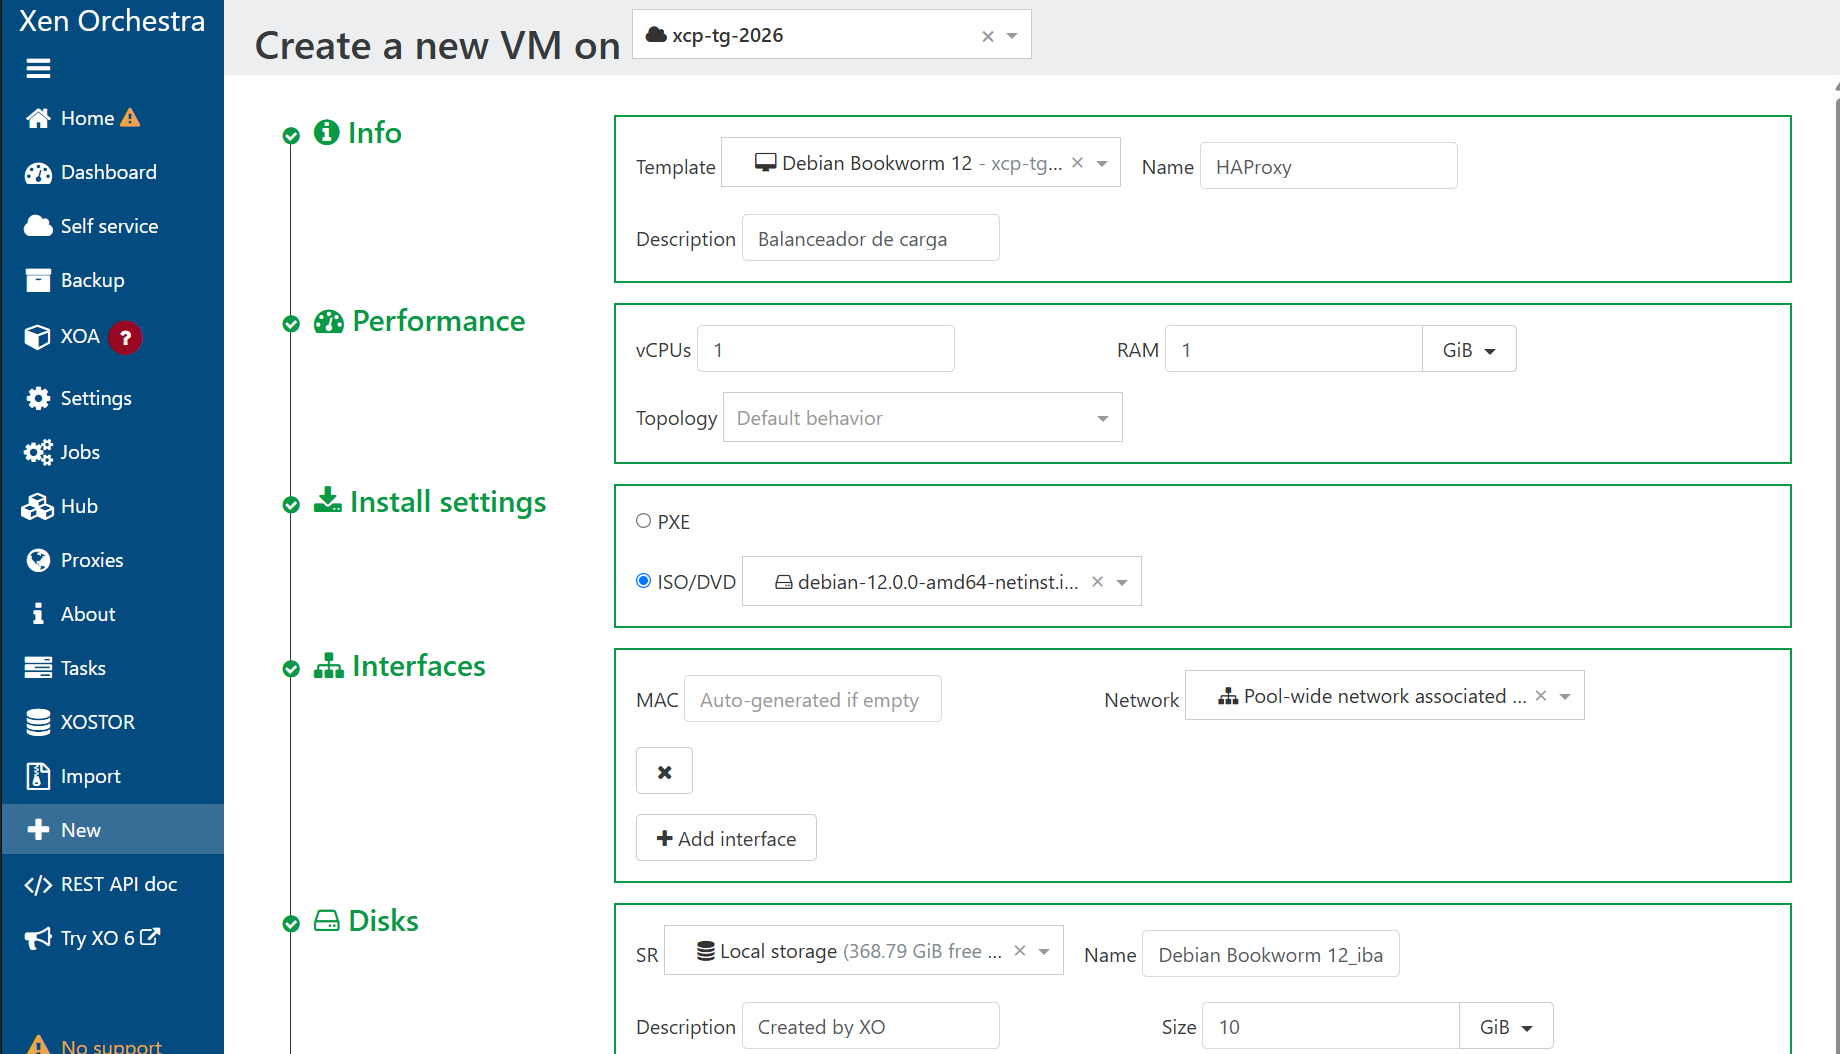
\includegraphics[width=0.8\textwidth]{mainmatter/II-desarrollo-metodologico/implementacion/imagenes/configuracion-vm-haproxy.png}
	\caption{Configuración de la máquina virtual destinada a la implementación de HAProxy}
	\label{fig:configuracion-vm-haproxy}
\end{figure}

Posteriormente, se realizó la instalación del sistema operativo y la configuración de la interfaz de red, asignando la dirección \acs{IP} 172.30.30.66 al servidor. Esta dirección permite identificar el balanceador dentro de la infraestructura y establecer la comunicación con los servidores FreeIPA. La configuración realizada se presenta en la \autoref{fig:configuracion-ip-haproxy}.

\begin{figure}[H]
	\centering
	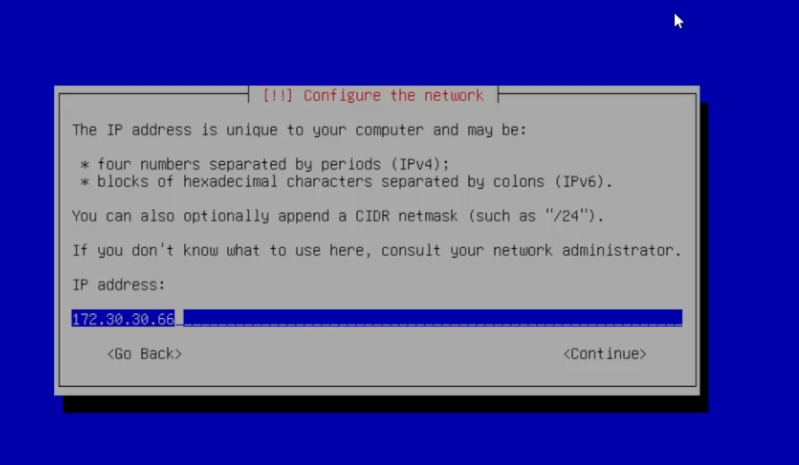
\includegraphics[width=0.8\textwidth]{mainmatter/II-desarrollo-metodologico/implementacion/imagenes/configuracion-ip-haproxy.png}
	\caption{Configuración de la dirección \acs{IP} del servidor HAProxy}
	\label{fig:configuracion-ip-haproxy}
\end{figure}

Una vez instalado y configurado el sistema operativo, se procedió con la instalación de HAProxy, estableciendo el componente encargado de recibir y gestionar las solicitudes dirigidas al servicio de directorio. En la \autoref{fig:instalacion-haproxy} se observa el proceso de instalación del balanceador.

\begin{figure}[H]
	\centering
	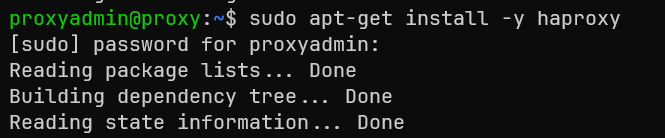
\includegraphics[width=0.8\textwidth]{mainmatter/II-desarrollo-metodologico/implementacion/imagenes/instalacion-haproxy.png}
	\caption{Instalación de HAProxy}
	\label{fig:instalacion-haproxy}
\end{figure}
Posteriormente, se configuró el archivo \texttt{/etc/haproxy/haproxy.cfg}, estableciendo los parámetros necesarios para que HAProxy pueda recibir y distribuir las conexiones del servicio de directorio tanto en su canal estándar como en su variante cifrada.

En primer lugar, para el tráfico \ac{LDAP} sin cifrado explícito, se definió el frontend \texttt{ft\_ldap}, encargado de recibir las conexiones en el puerto 389 mediante el modo \texttt{tcp} y con la opción \texttt{option tcplog} activada para el registro de tráficos. Este frontend transfiere las peticiones al backend \texttt{bk\_ldap}, donde se configuró el algoritmo \texttt{roundrobin} para distribuir la carga entre los servidores \texttt{ipa1} e \texttt{ipa2} (\texttt{ipa1.grid.uniquindio.edu.co} e \texttt{ipa2.grid.uniquindio.edu.co}). Asimismo, se incluyó la directiva \texttt{option ldap-check}, la cual realiza comprobaciones de salud específicas del protocolo \ac{LDAP} para determinar la disponibilidad de cada servidor antes de asignarle tráfico.

De forma complementaria, se estructuró la entrada para la comunicación cifrada \ac{LDAPS} mediante el frontend \texttt{ft\_ldaps}, configurado para recibir solicitudes en el puerto 636 bajo el modo \texttt{tcp}. Este remite las conexiones al backend \texttt{bk\_ldaps}, el cual balancea las peticiones cifradas entre los nodos \texttt{ipa1} e \texttt{ipa2} en el puerto 636 usando el algoritmo \texttt{roundrobin}. En este bloque, la validación de estado de los nodos se lleva a cabo mediante \texttt{option ssl-hello-chk}, asegurando que los servidores respondan adecuadamente al saludo inicial \ac{SSL}/\ac{TLS} antes de ser considerados operativos en el clúster. La configuración del frontend y backend utilizados para el balanceo se presenta en la \autoref{fig:configuracion-balanceo-freeipa-haproxy}.

\begin{figure}[H]
	\centering
	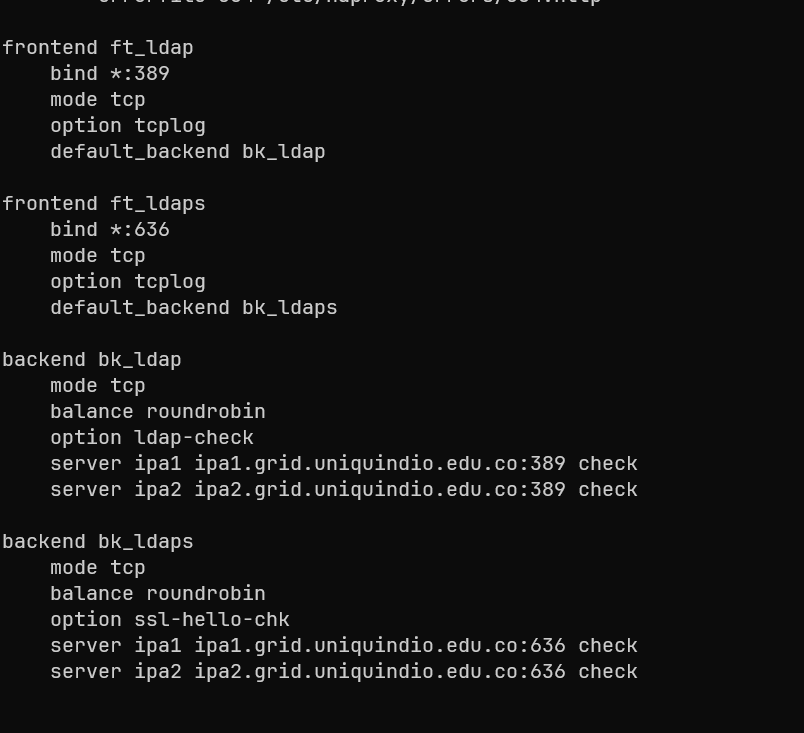
\includegraphics[width=0.8\textwidth]{mainmatter/II-desarrollo-metodologico/implementacion/imagenes/configuracion-balanceo-freeipa-haproxy.png}
	\caption{Configuración de HAProxy para el balanceo de los servidores FreeIPA}
	\label{fig:configuracion-balanceo-freeipa-haproxy}
\end{figure}

\subsection{Configuración del servicio \texorpdfstring{\acs{LDAP}}{LDAP} para el nombre virtual}

Para completar la integración entre HAProxy y FreeIPA, fue necesario registrar en FreeIPA el nombre \texttt{ipa.grid.uniquindio.edu.co} como un host. Este nombre representa el punto de acceso utilizado para el servicio de directorio a través del balanceador, diferenciándolo de los nombres individuales de los servidores \texttt{ipa1} e \texttt{ipa2}.

Para ello, se creó en FreeIPA un host fantasma (\textit{ghost host}) asociado al nombre \texttt{ipa.grid.uniquindio.edu.co}, utilizado para representar el nombre virtual mediante el cual se accederá al servicio de directorio a través de HAProxy. Para su creación se empleó el comando \texttt{ipa host-add} junto con los parámetros \texttt{-{}-random} y \texttt{-{}-force}. El parámetro \texttt{-{}-random} permite generar automáticamente una contraseña aleatoria para el host, mientras que \texttt{-{}-force} permite completar la creación del host fantasma bajo las condiciones requeridas por este procedimiento. Esta configuración permite registrar en FreeIPA el nombre virtual antes de asociarlo posteriormente con el servicio \ac{LDAP} utilizado por los servidores de la infraestructura. La creación del host fantasma se presenta en la \autoref{fig:creacion-host-servicio}.

\begin{figure}[H]
	\centering
	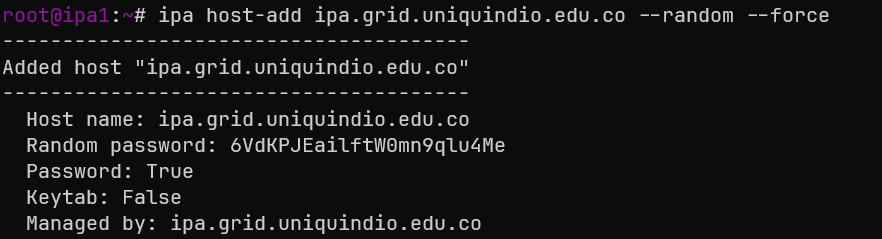
\includegraphics[width=0.8\textwidth]{mainmatter/II-desarrollo-metodologico/implementacion/imagenes/creacion-host-servicio.png}
	\caption{Creación del host destinado a la configuración del servicio}
	\label{fig:creacion-host-servicio}
\end{figure}

Una vez creado el host, se registró el servicio \ac{LDAP} asociado al nombre \nolinkurl{ipa.grid.uniquindio.edu.co} mediante el comando \texttt{ipa service-add}. Esta operación permite crear en FreeIPA el principal de servicio \nolinkurl{ldap/ipa.grid.uniquindio.edu.co@GRID.UNIQUINDIO.EDU.CO}, el cual identifica el servicio \ac{LDAP} que se utilizará bajo la identidad virtual. Esta configuración es fundamental para que la infraestructura de Kerberos y los mecanismos de autenticación de FreeIPA reconozcan correctamente el servicio, independientemente del servidor físico que atienda la solicitud. El proceso de adición del servicio se ilustra en la \autoref{fig:adicion-servicio-host}.

\begin{figure}[H]
	\centering
	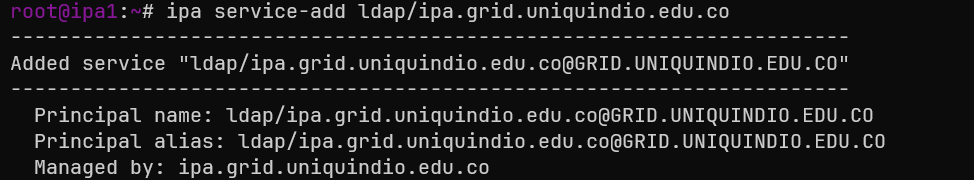
\includegraphics[width=0.8\textwidth]{mainmatter/II-desarrollo-metodologico/implementacion/imagenes/adicion-servicio-host.png}
	\caption{Adición del servicio al host configurado}
	\label{fig:adicion-servicio-host}
\end{figure}

Posteriormente, el servicio \ac{LDAP} se asoció tanto al servidor principal ipa1 como al servidor de réplica ipa2. De esta manera, ambos servidores quedan registrados como miembros del mismo servicio \ac{LDAP}, permitiendo que el nombre virtual utilizado por los clientes pueda ser atendido por cualquiera de los dos nodos de FreeIPA. Esta configuración constituye un mecanismo de redundancia para el acceso al servicio de directorio, ya que vincula el servicio lógico \nolinkurl{ldap/ipa.grid.uniquindio.edu.co} con los dos servidores que se encuentran detrás de HAProxy. La incorporación del servicio en ambos servidores se observa en la \autoref{fig:incorporacion-servicio-freeipa}.

\begin{figure}[H]
	\centering
	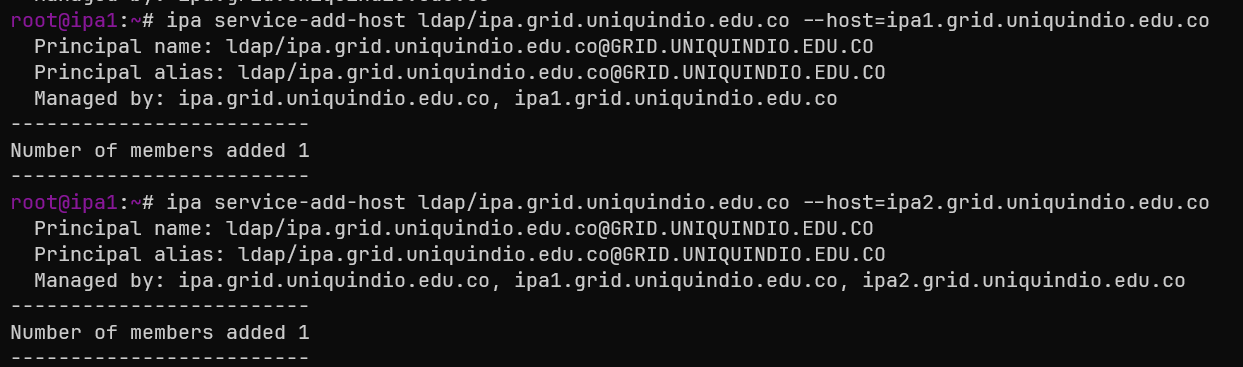
\includegraphics[width=0.8\textwidth]{mainmatter/II-desarrollo-metodologico/implementacion/imagenes/incorporacion-servicio-freeipa.png}
	\caption{Incorporación del servicio en los servidores FreeIPA}
	\label{fig:incorporacion-servicio-freeipa}
\end{figure}

Posteriormente, se verificó la configuración del servicio mediante la consulta de sus propiedades en FreeIPA. Esta comprobación permitió confirmar que el principal \ac{LDAP} había sido creado correctamente y que los servidores ipa1 e ipa2 se encontraban asociados al servicio. El resultado de esta verificación se presenta en la \autoref{fig:verificacion-servicio-ldap-virtual}.

\begin{figure}[H]
	\centering
	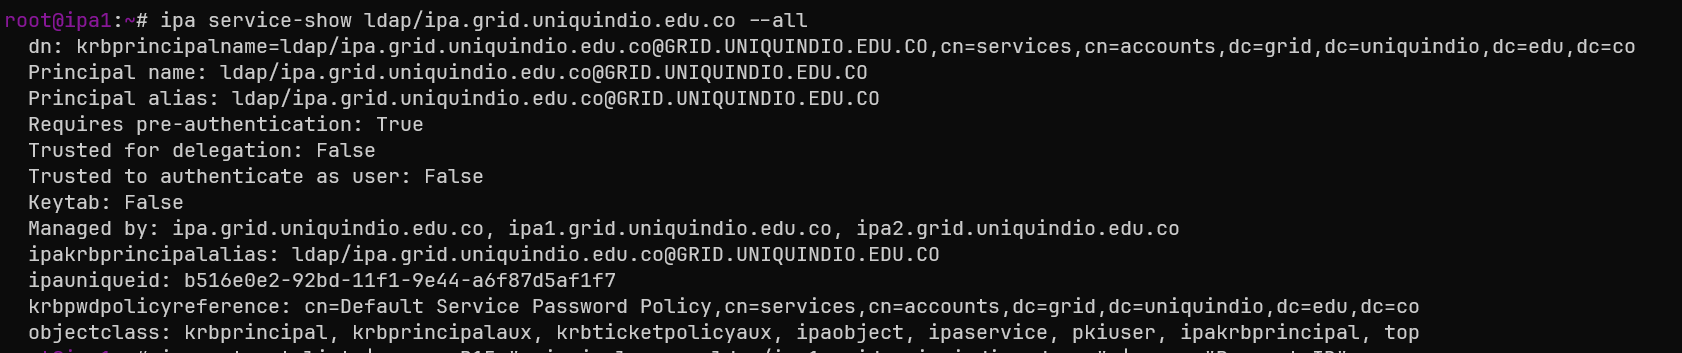
\includegraphics[width=0.8\textwidth]{mainmatter/II-desarrollo-metodologico/implementacion/imagenes/verificacion-servicio-ldap-virtual.png}
	\caption{Verificación del servicio \acs{LDAP} configurado para el nombre virtual}
	\label{fig:verificacion-servicio-ldap-virtual}
\end{figure}

\subsection{Configuración y validación de certificados}

Como parte de la configuración del acceso al servicio mediante el nombre virtual, se procedió a verificar y gestionar los certificados asociados a los servidores FreeIPA. Este procedimiento es necesario porque las conexiones \ac{LDAP} protegidas mediante \ac{TLS} utilizan el certificado digital del servidor para validar su identidad y, por tanto, el nombre utilizado para establecer la conexión debe estar contemplado en el certificado.

En el servidor principal se consultó la solicitud de certificado correspondiente al servicio y posteriormente se realizó su actualización mediante ipa-getcert. En este proceso se incluyó ipa.grid.uniquindio.edu.co como nombre \ac{DNS} asociado al certificado, además del nombre propio del servidor. Esto permite que el certificado pueda ser validado cuando la conexión se realice utilizando el nombre virtual definido para el servicio. En la \autoref{fig:certificado-servicio-servidor-principal} se observa la solicitud y el estado de monitorización del certificado en ipa1.

\begin{figure}[H]
	\centering
	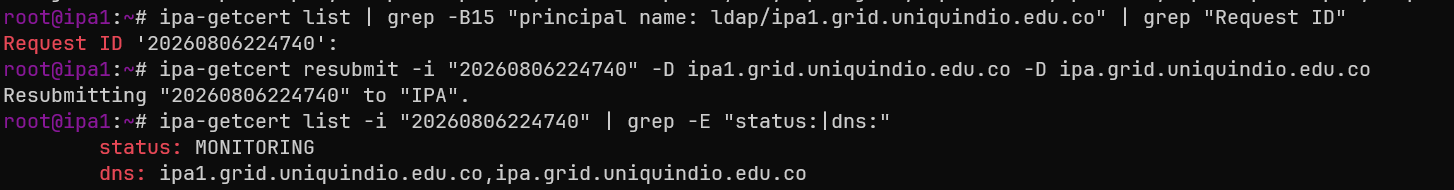
\includegraphics[width=0.8\textwidth]{mainmatter/II-desarrollo-metodologico/implementacion/imagenes/certificado-servicio-servidor-principal.png}
	\caption{Configuración y verificación del certificado del servicio en el servidor principal}
	\label{fig:certificado-servicio-servidor-principal}
\end{figure}

Finalmente, se realizó el mismo procedimiento en el servidor de réplica ipa2, verificando que el certificado asociado incluyera el nombre virtual utilizado para el servicio. La comprobación del estado MONITORING permite verificar que FreeIPA continúa gestionando la solicitud de certificado y que los nombres \ac{DNS} asociados al certificado corresponden a los nombres definidos para la infraestructura. La verificación realizada en el servidor de réplica se presenta en la \autoref{fig:certificado-servicio-servidor-replica}.

\begin{figure}[H]
	\centering
	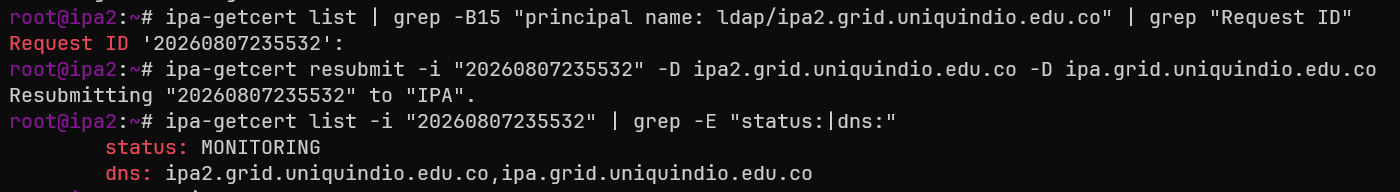
\includegraphics[width=0.8\textwidth]{mainmatter/II-desarrollo-metodologico/implementacion/imagenes/certificado-servicio-servidor-replica.png}
	\caption{Configuración y verificación del certificado del servicio en el servidor de réplica}
	\label{fig:certificado-servicio-servidor-replica}
\end{figure}
